\chapter{Technical Foundations and Possible Models}
\label{ch:foundations}

In the failed insertion shown in Chapter~\ref{ch:reassemble}, the first camera frame carried the same
weight as the last. From that recording, the visual
model took 16 frames and averaged their features into a single description of the
action. Reading the frames in reverse order would have given exactly the same
description. For an insertion, this matters. A change near the point of contact may be
visible in only a few frames, and averaging over the whole action can reduce its
influence.

The robot also recorded force, torque, and movement during the insertion. These
measurements offered a second view of the same event. The main REASSEMBLE experiment
first made a prediction from the camera and another from the sensors. It then tested
whether combining the two helped identify failed actions. The recorded failure label
made that comparison possible, even though the physical cause of this particular failure
was unknown.

PHM raised a different question. There, the aim was to predict a numerical indicator of
gear condition from machine measurements. Photographs taken after a run supplied the
target for the main sensor study. A photograph used to define what a model should
predict has a different role from a camera frame supplied to a model when it makes a
prediction. That distinction affects what can be claimed from the fusion experiments in
Chapters~\ref{ch:phm} and~\ref{ch:reassemble}.

\section{What the models predicted}

In REASSEMBLE, each completed action had one recorded outcome: success or failure. The
16 frames from the insertion therefore belonged to \textbf{one prediction}. Treating
them as 16 separate test cases would count the same outcome 16 times. A recording could
also contain several actions carried out under similar conditions. For this reason, the
evaluation kept actions from the same recording together when separating training and
assessment data.

Failure was the positive outcome in REASSEMBLE, ViFailback, and HANDOVER. In MSM, the
positive outcome was an abnormal cutting interval under the label definition used in
that study. PHM used regression because its target was a number. A low error in PHM
meant that a prediction was close to the indicator derived from the photographs.
Establishing how closely that indicator measured actual tooth damage would require an
independent physical measurement.

HANDOVER supplies supporting unimodal and fixed-average results in
Appendix~\ref{app:handover}. Its missing participant-to-trial mapping prevented the
mandatory participant-safe OOF construction for learned fusion, so the presence of
paired modalities alone did not make a fitted stacker eligible.

For the REASSEMBLE insertion, let \(p_v\) be the failure probability estimated from
video and \(p_s\) the probability estimated from sensors. Both estimates refer to the
same action. Their values can differ because the models receive different measurements
and learn different relationships from the training data.

A classification model produces a score. A sigmoid function turns that score into a
value between zero and one. Whether the value is a good probability estimate is a
separate issue. For example, if a model gives many actions a failure probability close
to 0.8, about eight in ten of those actions should fail if the model is well calibrated
in that range. This chapter distinguishes models that combine probabilities directly
from models that first convert them to \textit{log-odds}, using
\(\ell(p)=\log[p/(1-p)]\). The software clips probabilities near zero and one so this
calculation remains defined.

\section{What the camera contributed}

The REASSEMBLE visual model began with a detector trained to find objects in images.
RT-DETR has a convolutional backbone that extracts image features at several scales. Its
hybrid encoder combines information across those scales. A decoder and detection heads
then use the features to predict object classes and bounding boxes
\parencite{Zhao2024RTDETR}. For the insertion study, the available label described
whether the action succeeded. There was no target box marking the place where it failed.

The main experiment used the ResNet18-vd backbone from the
\texttt{PekingU/rtdetr\_r18vd} checkpoint. Its weights stayed fixed. Each hand-camera
frame used the shared RGB preprocessing specified in
Appendix~\ref{app:implementation}, Section~\ref{sec:rtdetr-preprocessing}.

For each frame, the backbone returned three feature maps. A feature map records how
strongly an image feature responds at different positions. The model took the average
response across each map channel and joined the results. This gave 896 numbers per
frame. Averaging those numbers across the 16 selected frames produced 896 numbers for
the completed action. A separately trained classification head used them to estimate the
probability of failure. The detector’s hybrid encoder, decoder, and bounding-box heads
were bypassed in this experiment.

Two details of the insertion disappear during those averages. The first is the exact
position of a feature in the image. The second is when that feature appeared. For
example, one feature might respond strongly in a frame near contact and weakly in the
other frames. Its average could be the same as a moderate response spread across several
frames. The resulting 896 values would not tell the prediction head which pattern had
occurred.

This limitation led to a specific comparison in Chapter~\ref{ch:reassemble}. The main model averaged
frames across the whole action. A later experiment pooled features from the last four of
the sixteen sampled frames, giving the final part of the movement its own
representation. Both models answered a question about a completed action. Testing an
early warning would require an earlier decision time and would exclude every frame
recorded after it.

Previous studies give reasons to compare these choices. Pretrained convolutional
features have been useful in industrial inspection \parencite{Roth2022Towards}, and the
Vision Transformer study showed that the amount of pretraining data affects the
comparison between convolution and attention \parencite{P010}. Video Swin keeps local
information across both space and time, with a computing cost that depends on the clips
and image crops used \parencite{P013}. TimeSformer reported an advantage for separate
spatial and temporal attention on Kinetics-400 and Something-Something V2
\parencite[Table~1]{P034}. The question for REASSEMBLE was narrower: with the available
recordings and training time, did retaining a selected part of the action help predict
its outcome?

PHM also used a model from the RT-DETR family, but its implementation followed a
different route. The software ran a frozen RT-DETR-L detector and collected three
intermediate feature maps during its prediction process. Pooling these maps produced 768
image features. The software added the time taken to extract them, so the regression
head received \textbf{769 inputs}. Any interpretation of this image experiment must
account for that timing value as well as the photograph.

Keeping an encoder frozen also allowed its features to be saved and reused across
training splits. Later experiments investigated what changed when the visual features
themselves were allowed to adapt. In ViFailback, the study distinguished a generic model
pretrained on COCO, a model previously trained with REASSEMBLE labels, and the completed
stages of training on the target task. These models had different training histories.
Comparing their epoch counts alone would miss differences in batch size, learning rate,
image augmentation, and early stopping. Where the record contains only saved features,
it confirms feature extraction. A claim about classification or fusion also requires a
completed assessment.

\textit{Implementation records: \EvidenceRef{E064}{}, \EvidenceRef{E065}{}, \EvidenceRef{E033}{}.}

\section{What the machine sensors contributed}

During a REASSEMBLE action, the robot recorded 22 channels: three force channels, three
torque channels, two gripper channels, seven joint-effort channels, and seven
joint-velocity channels. A brief change in force and a gradual rise in force can have
the same average. The sensor study therefore compared two ways of reading the same
measurements. One described the action with a small set of statistics. The other learned
from short, overlapping parts of the signal.

For the statistical model, each channel supplied ten values: the mean, standard
deviation, median, minimum, maximum, lower and upper quartiles, range, root-mean-square
amplitude, and slope over action progress. Together, the 22 channels produced
\textbf{220 features per action}. For a force channel, the maximum retained the highest
value in the resampled force channel. The range described the distance between its
lowest and highest values. The slope described whether force generally rose or fell as
the action progressed. None of these values, on its own, identified the moment when the
highest force occurred.

These simple features were a serious comparison for the learned model. They captured
useful properties of the robot’s movement, and their compact size made them a practical
reference with the available training data. Other industrial work has likewise shown
that carefully chosen features can compete with learned representations, including in 3D
anomaly detection \parencite{Horwitz2023Back}.

The second sensor model used PatchTST. To prepare its input, each completed action was
represented by 512 positions from start to finish on each of the 22 channels. Position
256 was therefore near the middle of the action, whether that action lasted a few
seconds or much longer. The spacing was measured in \textbf{action progress}. Two
neighbouring positions did not necessarily represent the same number of milliseconds in
different actions. This matters if the signal is later interpreted in terms of physical
vibration frequencies.

Figure~\ref{fig:sensor-patch-tokens} shows how overlapping sensor patches become tokens.

\begin{figure}[htbp]
\centering
\caption{How overlapping sensor patches become tokens}
\label{fig:sensor-patch-tokens}
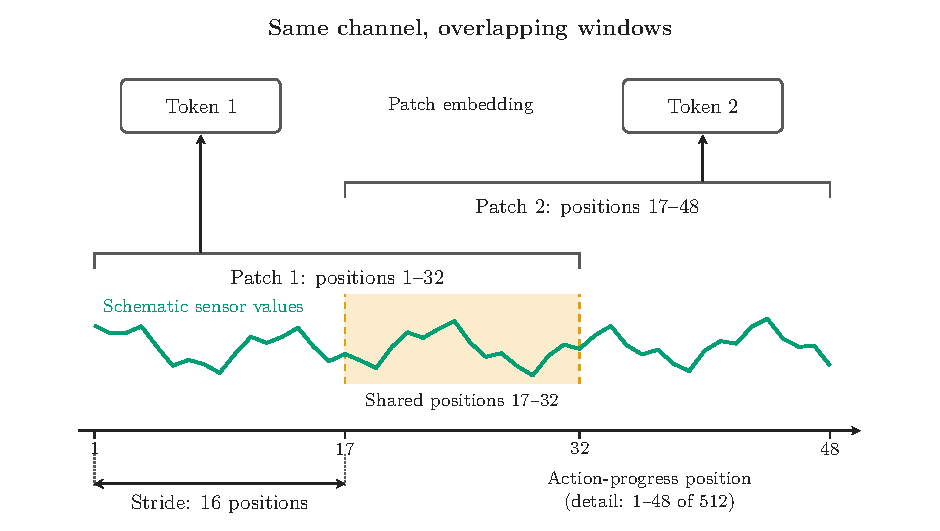
\includegraphics[width=\linewidth]{figures/review_explanatory_20261126/sensor_patch_tokens.pdf}
\displaynote{One schematic REASSEMBLE sensor channel is shown from an action resampled
to 512 positions across 22 channels. Patches 1--32 and 17--48 share positions 17--32;
their starts are 16 positions apart. Each patch becomes a separate Transformer input,
called a \textit{token}.}
\end{figure}

The original PatchTST model processes each channel separately and shares its learned
weights across channels \parencite{Nie2023PatchTST}. This lets it learn from
neighbouring measurements without treating every single measurement as a separate token.
The published model addressed forecasting. In REASSEMBLE, the encoder was trained from
scratch to classify the outcome of a completed action.

The REASSEMBLE model used a patch width of 32, a stride of 16, a hidden width of 32, two
Transformer layers, four attention heads, and a feed-forward width of 64. With no
padding, 512 positions give 31 patches. The number actually processed depends on how the
software handles the end of the sequence. After encoding, the model averaged the patch
features, joined the channel representations, and projected the result to 128 values.
The inputs had already been standardised before entering the model, so internal scaling
was switched off. The software also received a mask identifying observed values. The
effect of a missing value depends on where the model actually applies that mask.

PHM used a separate patch-based model for minute-level sequences of different lengths.
Its default patches were 16 positions wide and started eight positions apart. A patch
was accepted if it contained at least one valid position. The model then used a mask
when pooling the outputs. The length of the sequences in a batch may affect the PHM
patch grid. Its effect on the reported results has not been measured. An optional output
head predicted a sorted profile through positive increments. Once the values were
sorted, the output could describe the profile, but an individual value could no longer
be assigned to a particular tooth.

Other time-series studies help put the comparison in context. TS2Vec found that
replacing its convolutional encoder with a Transformer did not consistently improve
classification \parencite{P012}. MOMENT studied a different training history: its
Transformer learned from several datasets by reconstructing hidden parts of a series
\parencite{P018}. The PatchTST results in this thesis apply to the training data and
budget used here. They leave open what a pretrained time-series encoder might achieve.

\begin{table}[htbp]
\centering
\caption{What reached the PHM and REASSEMBLE prediction heads}
\label{tab:ch3-representations}
\small\singlespacing
\setlength{\tabcolsep}{4pt}
\renewcommand{\arraystretch}{1.15}
\begin{tabularx}{\linewidth}{@{}P{0.26\linewidth}YY@{}}
\toprule
\textbf{Experiment} & \textbf{Input to the prediction head} & \textbf{What the model predicted} \\
\midrule
PHM image model & 768 pooled image features and one extraction-time value & A numerical target \\
PHM temporal model & Features from variable-length sequences of minute-level
measurements & A single value or an optional sorted profile \\
REASSEMBLE visual model & 896 features averaged across 16 hand-camera frames & Success
or failure of the completed action \\
REASSEMBLE statistical sensor model & 220 summary values from 22 channels & The sensor
probability used by the main fusion models \\
REASSEMBLE PatchTST model & 128 learned features from the same 22 channels & A separate
sensor-only prediction in the main comparison \\
\bottomrule
\end{tabularx}
\end{table}

The last two rows in Table~\ref{tab:ch3-representations} are important for interpreting
the experiments. Combining sensor statistics with PatchTST features tests whether two
descriptions of the \textbf{same measurements} work better together. Combining the
statistical sensor prediction with the camera prediction asks a different question:
whether a second physical source adds useful information.

\textit{Implementation records: \EvidenceRef{E031}{}, \EvidenceRef{E065}{}.
Appendix~\ref{app:implementation} gives the model settings.
Appendix~\ref{app:reproducibility} identifies the components used in each experiment.}

\section{What counted as a fair comparison}

In REASSEMBLE, an insertion and a placement did not carry the same risk of failure. The
retained data contained 243 failures in 1,156 insertions and 22 failures in 1,088
placements (Chapter~\ref{ch:reassemble}). A predictor that knew only the action type could therefore
assign a higher failure score to an insertion before using a single frame or force
reading. This is why an action-only reference matters. It measures how much can already
be predicted from the task the robot was asked to perform.

PHM needed a different reference. For a held-out gear run, the constant model returned
the mean target value from the training runs. A sensor model had to improve on that
estimate to show that its readings helped predict the photographic target. The training
mean has a specific mathematical property: among constant predictions, it gives the
smallest squared error on the training data. The median has the corresponding property
for absolute error. The main PHM experiment used the mean.

\begin{table}[htbp]
\centering
\caption{Reference predictions used to judge the models}
\label{tab:ch3-reference-predictors}
\small\singlespacing
\setlength{\tabcolsep}{4pt}
\renewcommand{\arraystretch}{1.15}
\begin{tabularx}{\linewidth}{@{}P{0.28\linewidth}Y@{}}
\toprule
\textbf{Reference} & \textbf{What the comparison asks} \\
\midrule
Training mean & Do PHM measurements predict the gear-condition proxy better than the
same fixed value for every run? \\
Class frequency or action context & How much can already be predicted from the training
failure rate or the type of action? \\
Ridge or logistic regression & What can a regularised model learn from compact features?
Ridge predicts a number. Logistic regression predicts a binary outcome. \\
Single-input neural head & How well does the camera or temporal sensor model perform on
its own on the assessment cases? \\
Histogram gradient boosting & Does the result also hold against a nonlinear sensor
predictor built from decision trees? \\
\bottomrule
\end{tabularx}
\end{table}

The main REASSEMBLE sensor predictor used logistic regression on the 220 statistics. It
learned a coefficient for each feature and an intercept. The study selected its
regularisation setting from 0.1, 1, and 10 within the training partitions. The F2 fusion
model also used logistic regression, but its regularisation setting was fixed at 1. Only
the sensor model selected among those three values.

The visual head and the PatchTST classifier used class-weighted binary cross-entropy.
This allowed failures and successes to carry different weights during fitting. The
original context gates used the unweighted form of the loss. The visual head had 114,945
trainable parameters above the frozen backbone. The PatchTST sensor model had 109,505,
including 90,369 in its projection and classifier. Although the totals were close, the
visual backbone had already been pretrained, whereas the temporal encoder had to learn
from the study data.

ViFailback and MSM also used histogram gradient boosting as a sensor reference. This
method combines decision trees and can learn relationships that a linear model misses.
ViFailback selected a candidate through its validation procedure. The MSM result came
from its own controller-feature protocol. Appendix~\ref{app:implementation} records the
settings for each study.

\section{How the models combined their inputs}

For the REASSEMBLE insertion, the main fusion models received just two numbers from the
prediction branches: the calibrated camera probability \(p_v\) and the calibrated sensor
probability \(p_s\). By this point, the camera branch had already averaged the frames,
and the sensor branch had already reduced the signals to 220 statistics. A fusion model
could change how much it used each prediction. It could not go back to a particular
frame or inspect the force reading at the moment of contact.

Figure~\ref{fig:fusion-interfaces} shows the inputs to the REASSEMBLE stacker and context gates.

\begin{figure}[H]
\centering
\caption{Inputs to the REASSEMBLE stacker and context gates}
\label{fig:fusion-interfaces}
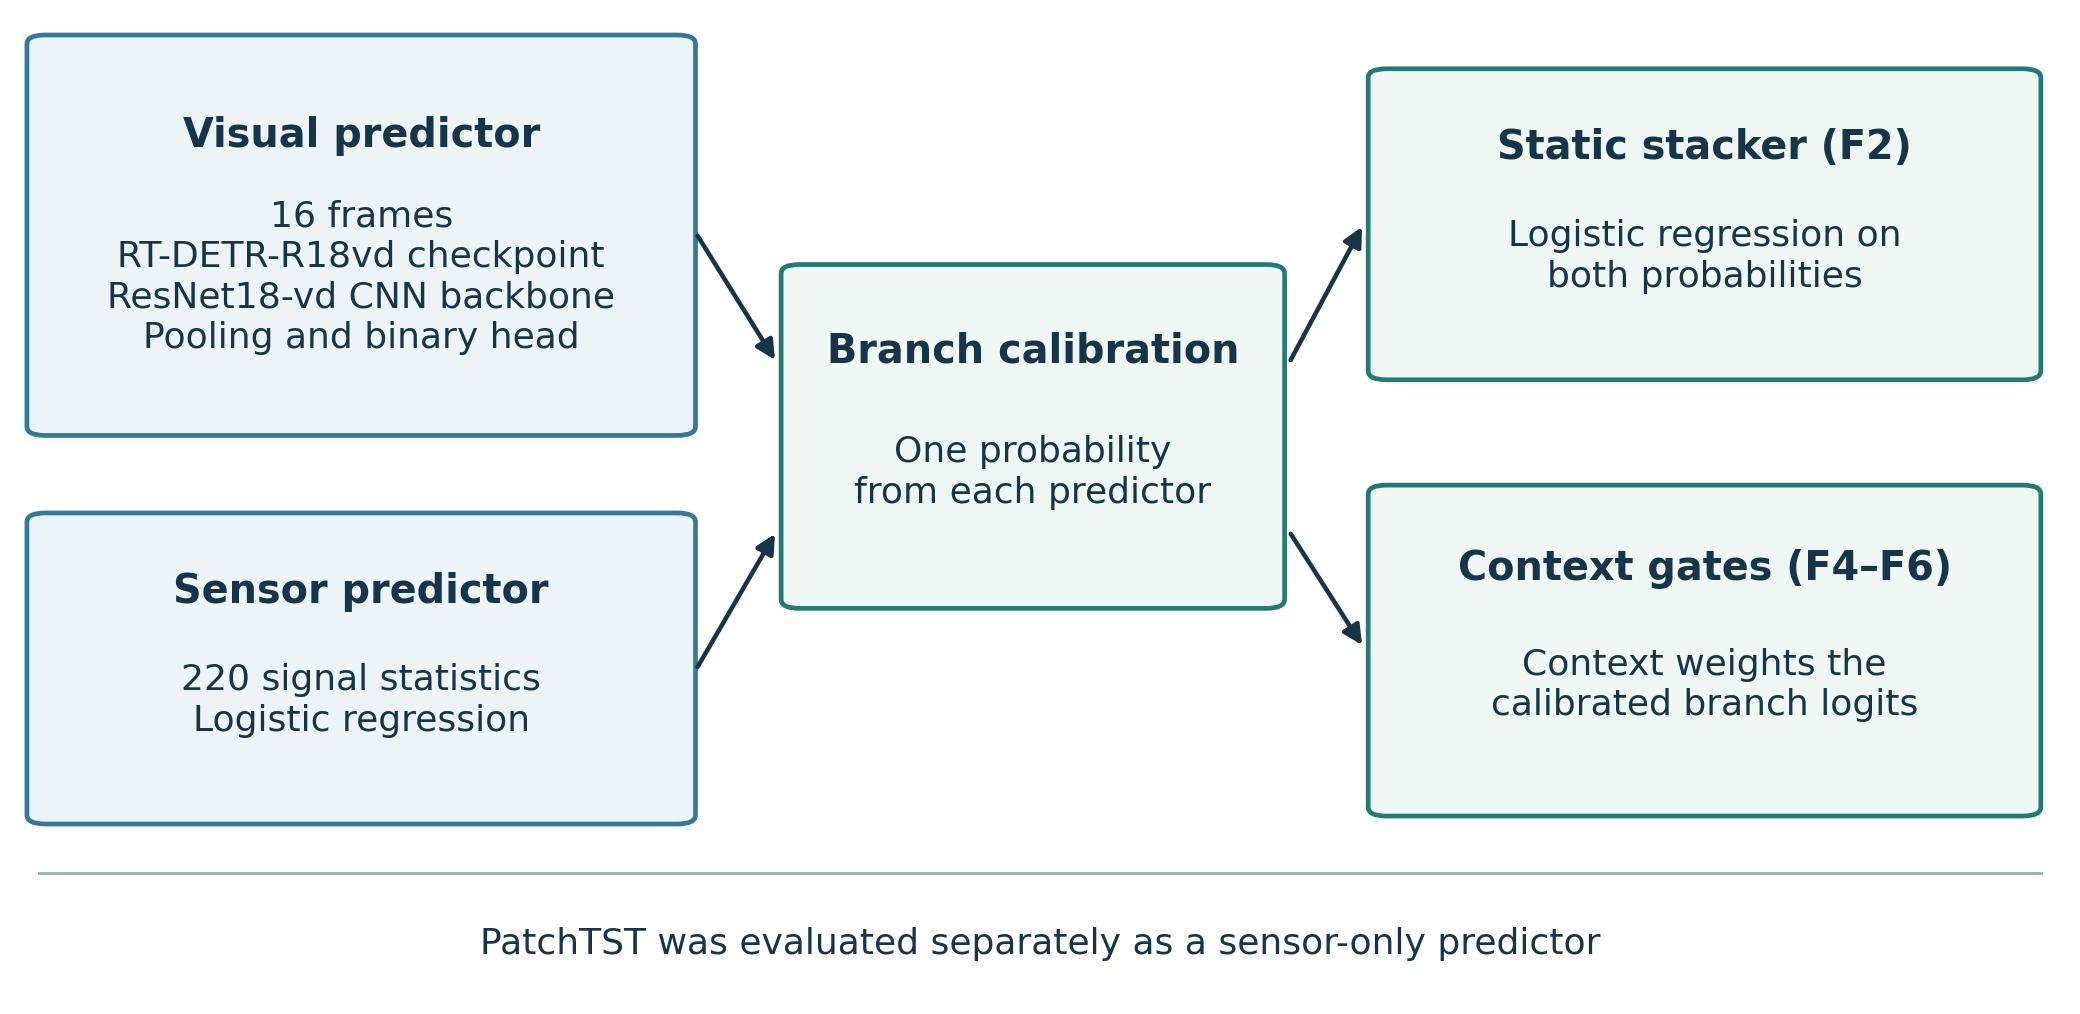
\includegraphics[width=\linewidth]{figures/fusion_interfaces}
\displaynote{The 16 camera frames produced one calibrated prediction. Logistic
regression on the 220 sensor statistics produced the other. F2 used the two
probabilities directly. F4--F6 converted them to log-odds and combined them using
context. PatchTST was evaluated separately as a sensor-only model.}
\end{figure}

\subsection{Feature concatenation in PHM}
\label{sec:ch3-phm-feature-fusion}

PHM combined information at an earlier stage. Its \texttt{fused\_all\_three} model
joined learned features from three groups: process context, root-mean-square vibration
measurements, and condition indicators. One regression head then predicted the target
from the joined features. The software class was called \texttt{LateFusionRegressor},
but the values being joined were features. All three groups came from sensor or process
data. The photographs supplied the target for this comparison. Also, joining features
can increase the number of trainable parameters, so a change in error may reflect both
the extra information and the larger model. \textit{Implementation record:
\EvidenceRef{E004}{Section~12.4}.}

Figure~\ref{fig:workflow-phm-feature-fusion} shows this workflow.

\begin{figure}[H]
\centering
\caption{PHM feature-concatenation workflow}
\label{fig:workflow-phm-feature-fusion}
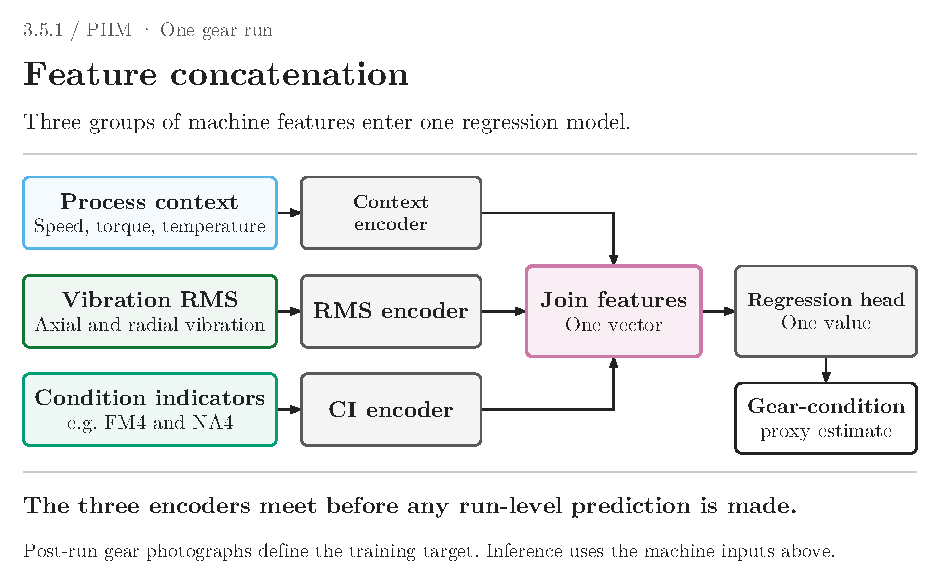
\includegraphics[page=1,width=\linewidth]{figures/fusion_workflows_20261126.pdf}
\displaynote{The inputs are engineered machine features. Post-run photographs define the
condition-proxy target. Here CI denotes condition indicators.}
\end{figure}

\subsection{Equal averaging (F1)}
\label{sec:ch3-equal-averaging}

The simplest REASSEMBLE fusion rule, F1, took the arithmetic mean of \(p_v\) and
\(p_s\). An increase of 0.1 in either branch raised the combined probability by 0.05.
The rule learned no combination weights. The branch models and their calibration still
had to be fitted on training data, and the calibration of their average still needed to
be checked.

Figure~\ref{fig:workflow-equal-averaging} shows this workflow.

\begin{figure}[H]
\centering
\caption{Equal-averaging workflow (F1)}
\label{fig:workflow-equal-averaging}
\includegraphics[page=2,width=\linewidth]{figures/fusion_workflows_20261126.pdf}
\end{figure}

\subsection{Logistic stacking (F2)}
\label{sec:ch3-logistic-stacking}

F2 learned a fixed combination from training predictions. It fitted an intercept \(b\),
a camera coefficient \(\alpha_v\), and a sensor coefficient \(\alpha_s\):

\begin{equation}
p_{\mathrm{F2}}=\operatorname{sigmoid}(b+\alpha_v p_v+\alpha_s p_s).
\label{eq:f2}
\end{equation}

The two coefficients can have different sizes or signs. Within each fitted model, the
same coefficients apply to every action. Their values describe how F2 used the two
branch scores. They cannot identify which physical event caused an insertion to fail.

Figure~\ref{fig:workflow-logistic-stacking} shows this workflow.

\begin{figure}[H]
\centering
\caption{Logistic-stacking workflow (F2)}
\label{fig:workflow-logistic-stacking}
\includegraphics[page=3,width=\linewidth]{figures/fusion_workflows_20261126.pdf}
\displaynote{The coefficients and intercept are fixed within each fitted model. Separate
assessment folds use separately fitted models.}
\end{figure}

Training F2 required care because its inputs were themselves model predictions.
Following the principle of stacked generalisation, the study used predictions for
training actions made by branches that had excluded the corresponding recording during
fitting \parencite{Ting1999Issues}. These \textit{out-of-fold predictions} formed the
prediction bank for the stacker. The outer assessment recordings stayed outside the
fitting process.

One dependence remained inside the training data. F2 reused the prediction bank for its
internal validation. A branch that produced a stacker-training score could therefore
have learned from recordings later used for stacker validation.
Chapter~\ref{ch:methodology} illustrates where this occurred. This detail matters
because using evaluation information to select a model can make its reported performance
look too favourable \parencite{P004}. The check must cover the whole procedure,
including preprocessing, calibration, and the construction of the prediction bank
\parencite{P017}.

\paragraph{Representation concatenation (F3).}
The REASSEMBLE F3 model combined the frozen visual head's 128-dimensional
representation with the 220 sensor statistics. Each input was standardised on the
fitting subset and passed through a separate learned 128-dimensional projection.
The concatenated representation was normalised and supplied to a fitted classifier
that predicted action failure. F3 therefore learned from representations rather than
from the two branch probabilities.\ev{Executed representation-concatenation model}
{\EvidenceRef{E048}{}, \EvidenceRef{E066}{}}

\subsection{Context-based gating (F4--F6)}
\label{sec:ch3-context-gating}

A fixed stacker applies the same rule to an insertion and a placement. The context gates
tested whether the rule should change from one action to the next. F4 received four
action indicators and two input-availability flags. F5 received 36 measures of input
quality and the two flags. F6 received all 42 values. For the recorded insertion, F4
could use the fact that the robot was inserting a part. F5 instead had access to the
measured properties of the inputs.

For an input \(m\), the gate used context \(u\) to produce a score \(q_m(u)\). The flag
\(a_m\) was one when the input was available and zero when it was missing. The gate
calculated a weight \(w_m\) for each available branch and combined the branch log-odds:

\begin{equation}
w_m(u,a)=
\frac{a_m\exp(q_m(u))}
{\sum_j a_j\exp(q_j(u))},
\qquad
p_G=\operatorname{sigmoid}\!\left(\sum_m w_m(u,a)\,\ell(p_m)\right).
\label{eq:gate}
\end{equation}

When both inputs were present, their weights added up to one. The original gates had no
free final intercept or further calibration step. F2, by comparison, learned an
intercept and operated directly on probabilities. A performance difference between F2
and a gate could therefore have several causes. To isolate the value of changing the
weights, the comparison also had to account for the score transformation, the training
loss, and the opportunity for recalibration.

Figure~\ref{fig:workflow-context-gating} shows this workflow.

\begin{figure}[H]
\centering
\caption{Context-based gating workflow (F4--F6)}
\label{fig:workflow-context-gating}
\includegraphics[page=4,width=\linewidth]{figures/fusion_workflows_20261126.pdf}
\end{figure}

Earlier fusion methods made other choices about \textit{where} the inputs could
interact. Gated Multimodal Units combined internal feature representations
\parencite{P006}. Multimodal attention bottlenecks allowed information to pass through
shared intermediate tokens \parencite{Nagrani2021MBT}. The REASSEMBLE gates had a
narrower task: they weighted two action-level predictions.

\subsection{Anchored adjustment and missing-input fallback}
\label{sec:ch3-anchored-adjustment}

A later experiment began with the fitted F2 stacker and asked whether a small adjustment
for each action could improve it. It kept F2’s intercept and branch coefficients. A
second network used context to multiply each coefficient by an adjustment:

\begin{equation}
p_A=\operatorname{sigmoid}\!\left[
b+\sum_m\alpha_m\{1+\tanh(h_m(u))\}p_m
\right].
\label{eq:anchored}
\end{equation}

Here \(h_m(u)\) is the adjustment-network output for branch \(m\). Its final layer
started at zero, so the model initially reproduced F2 exactly. For a finite output, the
multiplier lies between zero and two. The original coefficient keeps its sign. A control
model used a constant adjustment, which made it possible to test whether changing the
adjustment \textit{between actions} added value.

Figure~\ref{fig:workflow-anchored-adjustment} shows this workflow.

\begin{figure}[H]
\centering
\caption{Anchored-adjustment workflow}
\label{fig:workflow-anchored-adjustment}
\includegraphics[page=5,width=\linewidth]{figures/fusion_workflows_20261126.pdf}
\displaynote{Both inputs were available in the clean comparison. Known input loss used
the separate fallback described below.}
\end{figure}

There are theoretical conditions under which adaptive weighting can help
\parencite{Zhang2023QMF}. In practice, a quality measure must contain information about
when a branch prediction becomes less useful. An observed property of a force signal,
the confidence of the sensor model, and the accuracy of that confidence are three
different quantities. Calibration can also become worse when test conditions change
\parencite{P008}. A later quality-interaction experiment therefore compared prediction
heads with matched exposure to altered inputs during training. It was a separate study
from the original gate comparison.

The difference between a damaged signal and a missing signal is particularly clear in
REASSEMBLE. In one controlled test, six force and torque channels were fixed at their
training medians. The sensor input was still present. Its summaries and quality measures
were calculated again from the altered signals, and the fusion model still had to decide
how to use the sensor prediction. In a declared sensor outage, the evaluator already
knew the branch was missing. It returned the camera probability and used the camera
branch’s own decision threshold. If the camera alone was missing, it used the sensor
branch in the same way. If both were missing, it rejected the input.

With a declared outage, methods that return the same surviving prediction necessarily
give the same result for that action. Handling this case shows that the fallback rule
works as specified. Recognising that six \textit{present} channels have stopped carrying
useful information is a harder test. Research on ModDrop, EmbraceNet, and missing-input
Transformers gives further examples of training for incomplete inputs
\parencite{P005,P007,P016}.

\begin{table}[htbp]
\centering
\caption{Where the inputs met in each fusion method}
\label{tab:ch3-fusion-interfaces}
\small\singlespacing
\setlength{\tabcolsep}{4pt}
\renewcommand{\arraystretch}{1.15}
\begin{tabularx}{\linewidth}{@{}P{0.26\linewidth}YY@{}}
\toprule
\textbf{Method} & \textbf{Information available at the point of fusion} & \textbf{What
was learned} \\
\midrule
PHM feature concatenation & Features from three sensor-derived groups & A prediction
head fitted to the joined features \\
REASSEMBLE F1 & Two calibrated probabilities & The combination rule was fixed at equal weights. \\
REASSEMBLE F2 & The same two probabilities & One intercept and two coefficients shared
across actions \\
REASSEMBLE F3 & A 128-dimensional visual representation and 220 sensor statistics &
Separate projections and a classifier fitted to their concatenation \\
REASSEMBLE F4--F6 & Two branch logits, context, and availability flags & Weights that
could change from one action to the next \\
Anchored adjustment & Branch probabilities and context & Changes to the fitted F2
coefficients for each observation \\
\bottomrule
\end{tabularx}
\end{table}

\section{What the experiments can establish}

The main REASSEMBLE comparison used a frozen camera backbone, a statistical sensor
model, and fusion rules that combined their predictions. PatchTST remained a separate
sensor-only comparison on the same sensor measurements in the core study, and its
performance under a limited training budget leaves open what longer
training might achieve. Appendix~\ref{app:implementation} records the configurations,
and Appendix~\ref{app:reproducibility} identifies which prediction paths were actually
run.

The original research question also included sound. An Audio Spectrogram Transformer was
a possible way to represent it \parencite{P011}. Action-level audio prediction requires
reliable alignment between the sound and the labelled action. Chapter~\ref{ch:reassemble}
explains the decision to exclude audio from the predictive experiment. Its value for
these actions remains open.

The recorded insertion illustrates the boundary of the chapter’s claims. The model had
access to the whole action, so it could use visual evidence near the end. The sensor
model had access to the same action through force and movement measurements, but the
summaries it received had already lost much of the order of those measurements. The
fusion experiment could test whether combining those two predictions helped rank failed
actions on held-out recordings. It could not determine the physical cause of that
insertion failure or the earliest time at which the robot could have detected it.

The later experiments changed individual parts of that setup. Pooling the last four
sampled frames changed which frames contributed to the camera prediction. Longer
temporal training changed the opportunity given to the sensor model. Anchored adjustment
changed the fusion rule. The thesis did not run all three changes together. Each result
therefore belongs to the configuration that produced it. Chapter~\ref{ch:methodology}
describes the recording splits, training decisions, and assessment conditions needed to
read those results correctly.

\textit{Implementation records: \EvidenceRef{E112}{}, \EvidenceRef{E114}{}, \EvidenceRef{E110}{}.}
